\documentclass[10pt,a4paper]{article}
\usepackage[utf8]{inputenc}
%\usepackage[french]{babel}
\usepackage{tikz-network}
\usepackage{tikz}
\usepackage{graphics,multirow}
\usepackage{subcaption}
\usepackage{array}
\usepackage{xcolor}
\PassOptionsToPackage{hyphens}{url}
\usepackage{hyperref}
\usepackage{amsmath}
\usepackage{amsfonts}
\usepackage{amssymb}
\usepackage{mathtools}
\usepackage[total={6in,8in}]{geometry}
\usepackage[backend=biber,style=numeric,sorting=ynt]{biblatex}
\newcommand{\red}[1]{{\textcolor{red}{#1}}}
\newcommand{\green}[1]{{\textcolor{green}{#1}}}
\newcommand{\orange}[1]{{\textcolor{orange}{#1}}}
\addbibresource{report.bib}
 \hypersetup{
 %   bookmarks=true,         % show bookmarks bar?
 %   unicode=false,          % non-Latin characters in Acrobat’s bookmarks
 %   pdftoolbar=true,        % show Acrobat’s toolbar?
 %   pdfmenubar=true,        % show Acrobat’s menu?
 %   pdffitwindow=false,     % window fit to page when opened
 %   pdfstartview={FitH},    % fits the width of the page to the window
 %   pdftitle={My title},    % title
 %   pdfauthor={Author},     % author
 %   pdfsubject={Subject},   % subject of the document
 %   pdfcreator={Creator},   % creator of the document
 %   pdfproducer={Producer}, % producer of the document
 %   pdfkeywords={keyword1, key2, key3}, % list of keywords
 %   pdfnewwindow=true,      % links in new PDF window
    colorlinks=true,       % false: boxed links; true: colored links
    linkcolor=blue,          % color of internal links (change box color with linkbordercolor)
    citecolor=blue,        % color of links to bibliography
    filecolor=blue,         % color of file links
    urlcolor=blue        % color of external links
}
%% COLORS %%
%
\definecolor{mygreen}{RGB}{0,214,0}
%% MACROS %%

\newcommand\von{{\textsc{Von}}}
\newcommand\fon{{\textsc{Fon}}}
\newcommand\hon{{\textsc{Hon}}}
\newcommand\fston{$1^{\mathrm{st}}${\textsc{on}}}
\newcommand\nrep{N_{\mathrm{rep}}}
\newcommand\uprvec{\Pi_{\mathrm{Von}}^{\mathrm{U}}}
\newcommand\bprvec{\Pi_{\mathrm{1}}^{\mathrm{B}}}
\newcommand\hprvec{\Pi_{\mathrm{Von}}}
\newcommand\fprvec{\Pi_{\mathrm{1}}}
\newcommand\urank{K_{\mathrm{Von}}^{\mathrm{U}}}
\newcommand\brank{K_{\mathrm{1}}^{\mathrm{B}}}
\newcommand\hrank{K_{\mathrm{Von}}}
\newcommand\frank{K_{\mathrm{1}}}
\newcommand\vrank{K_{\mathrm{V}}}
\newcommand\reprank{K_{\mathrm{rep}}}
\newcommand{\tbd}[1]{\textcolor{blue}{{\textbf{To do: #1}}}}
\newcommand{\ask}[1]{\textcolor{red}{{\textbf{Question: #1}}}}
\newcommand\mems{\textit{memory nodes}}
\newcommand\kin{k_{\mathrm{in}}}
\newcommand\kout{k_{\mathrm{out}}}
\newcommand\uhonpr{Unbiased HON PR}
\newcommand\honpr{HON PR}
\newcommand\pr{1stON PR}
\newcommand\bpr{1stON Biased PR}
%\author{Célestin Coquidé}
\title{Complexity and Fitness of Methylated DNA sites and RNAs in the context of Breast Cancer Tissues}
\date{\today}
\begin{document}
\maketitle
\section{Aim of the study}
Highlighting the nestedness structure of the bipartite network representing correlations between methylated DNA sited and RNAs.
\section{Methods and Data}
\subsection{Nestedness}
Nested structures appear in the nature such that in ecological and socio-economic systems. In ecological systems, for instance, there is a nested distribution of species habitats. Where as some species only live in particular locations, some others live in a large variety of environments including those particular locations. In the context of network theory, a perfectly nested structure is such that for any pair of node ($i,j$) with $k_{i} < k_{j}$ their respective degree (number of neighbors), the set of nodes $i$ is interacting with is included in the set of nodes $j$ is interacting with. The adjacency matrix of such a network shows a triangular shape when columns and rows are sorted accordingly to the degree ordering of respective nodes. There are many metrics (other than degrees) permitting to infer the nested structure of a given network. Nestedness can appear in unipartite and bipartite networks. In the context of economical systems, especially the world trade network seen as a country-product bipartite network, recent research shows the existence of nestedness, see a complete review in \cite{mariani19}. In the context of biological systems nestedness structures have also been studied. In \cite{cantor17} different biological scales are considered. However, it seems that DNA-RNA interactions have not been studied yet. We choose the metric called fitness-complexity introduced in \cite{tacchella12} to investigate the nestedness structure of DNA-RNA bipartite network. Fitness and complexity is a non-linear and iterative algorithm permitting to infer the nestedness in bipartite network such as economical networks. In this context, the fitness is a country quality, and complexity is a product quality. In our approach we try to make an analogy where RNAs play the role of products and DNAs the role of countries. Here are the economical definitions of fitness and complexity.
\paragraph{Fitness and Complexity metrics}
\begin{equation}
\left\{
\begin{matrix}
F^{(n)}_{d} =  \sum_{r} B_{dr}Q^{(n-1)}_{r}\\
Q^{(n)}_{r} =  \frac{1}{\sum_{d}B_{dr}(1-F^{(n-1)}_{c})}
\end{matrix}
\right.
\label{eq:eq1}
\end{equation}
with $B_{dr}$ an element of the bi-adjacency matrix representing the correlation (positive or negative) interaction between a Methylated DNA $d$ and an RNA $r$, $F^{(n)}$ and $Q^{(n)}$ the Fitness and Complexity vector measured at iteration $n$.
\paragraph{Product's complexity}
\subsection{Data}
We used an open access cancer dataset from GDC Data Portal. From raw data consisting in methylated DNA and RNA's beta-values for up to 841 tumorous and normal breast tissues, we built a Matrix of Pearson Correlation Coefficients between Methylated DNA and RNA from these beta-values. A network representing the Pearson correlation coefficients between pairs (M-DNA,RNA) consists in a bipartite graph with coefficients as weight of the links containing. We also project DNAs into spacial clusters of length 40K base-pairs, this turns $N_{DNA} = 364285$ DNAs into a set of $N_{cl} = 93690$ clusters. The nature of correlations are either positive or negative.

We propose to measure complexity of RNAs from the complexity-fitness metric proposed in \cite{tacchella12}.
\section{The case of ESR1 synthesis and regulation}
The set of ESR1 synthesis and regulation consists in 508 RNAs and 4959 clusters of DNAs. We first construct the Pearson correlation matrix between clustered DNAs and RNA then we measure the complexity and fitness of nodes from the sub network related to the ESR1 regulation sub set.
\begin{figure}[h!]
%\begin{center}
\begin{center}
\resizebox{0.7\columnwidth}{!}{%
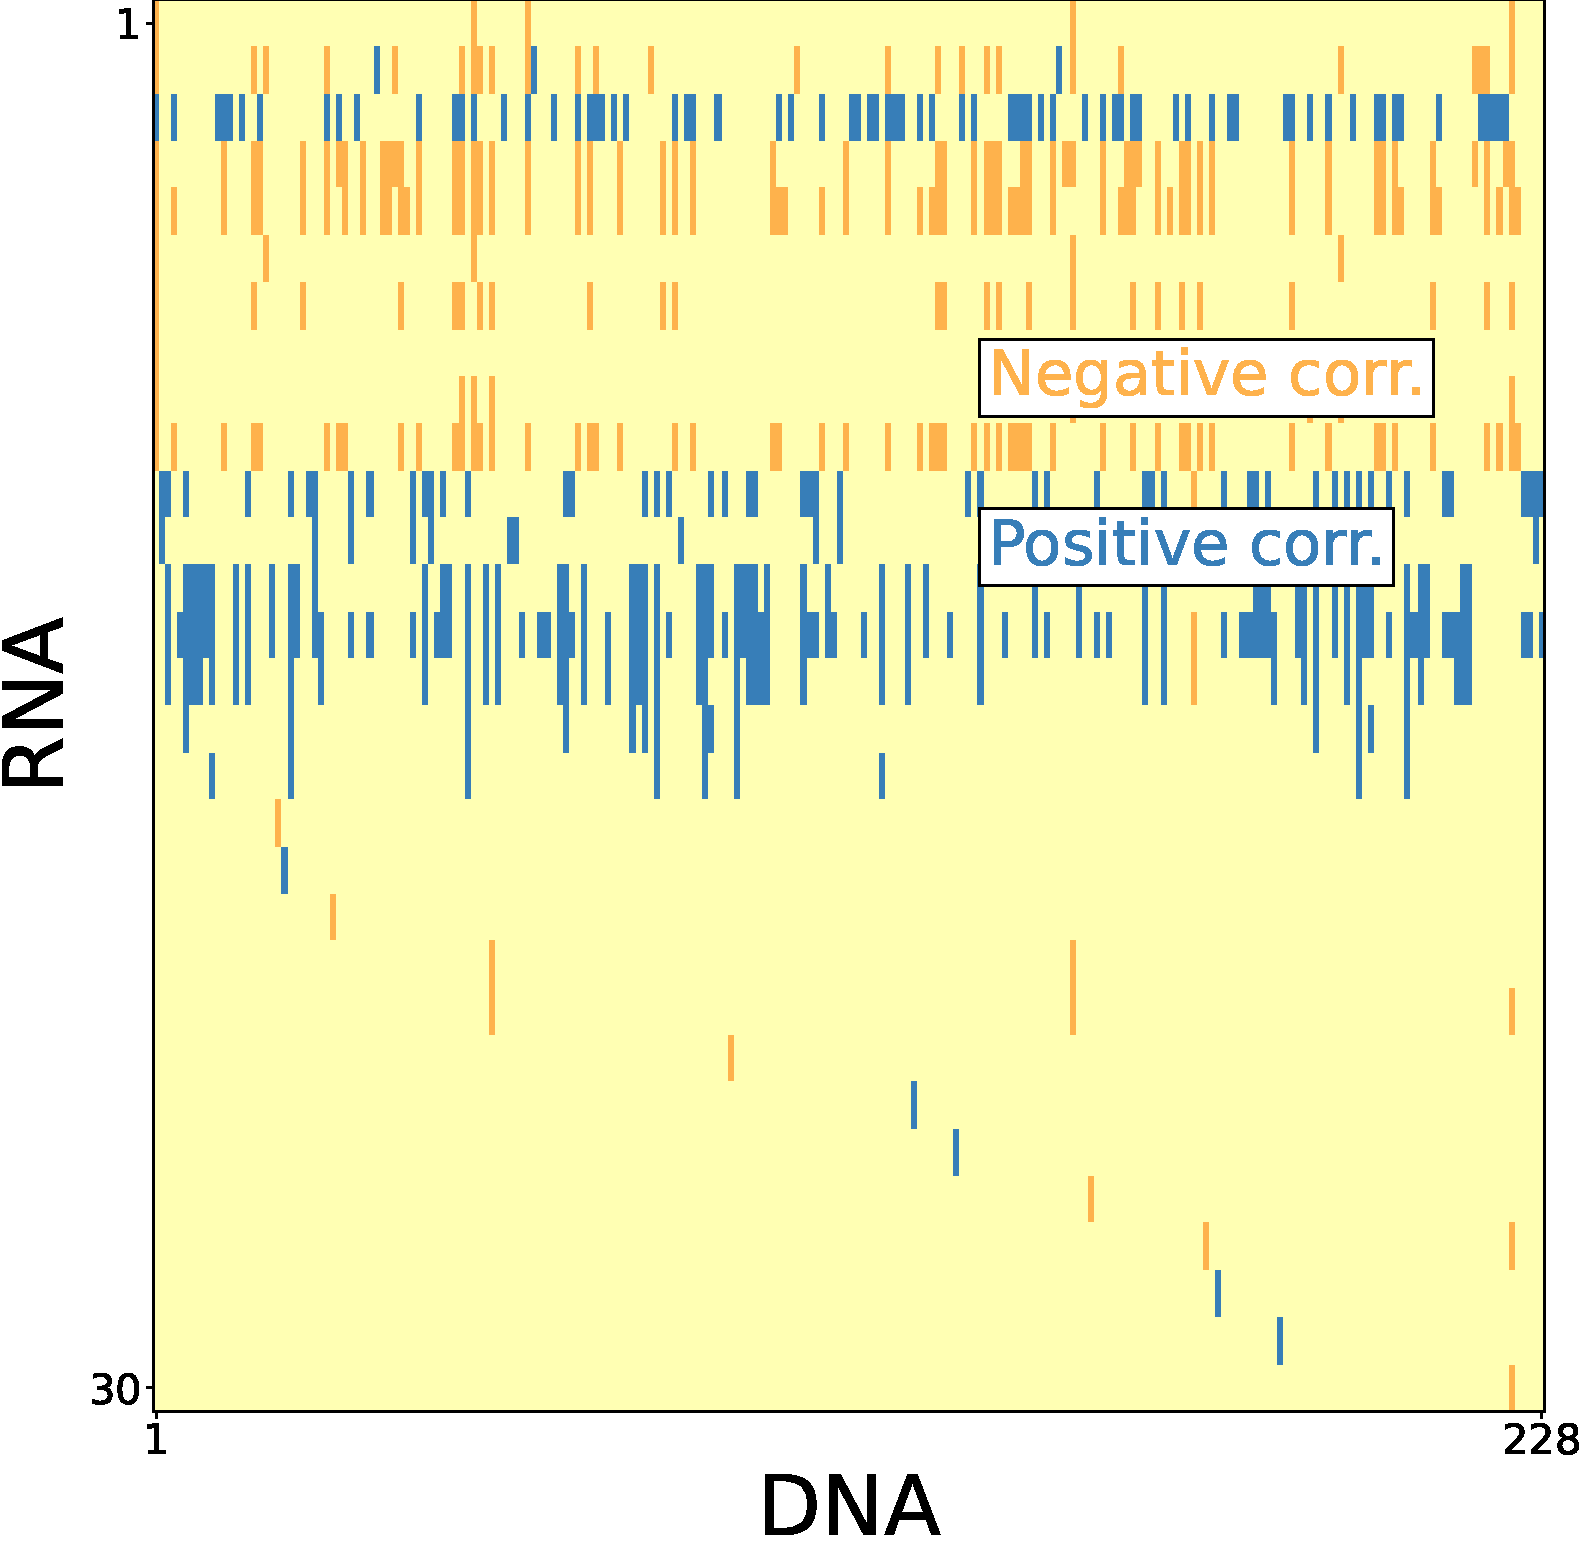
\includegraphics[width=0.5\columnwidth]{FIG/ADN_c-ARN_Matrix-unit-0.7-PN.pdf}
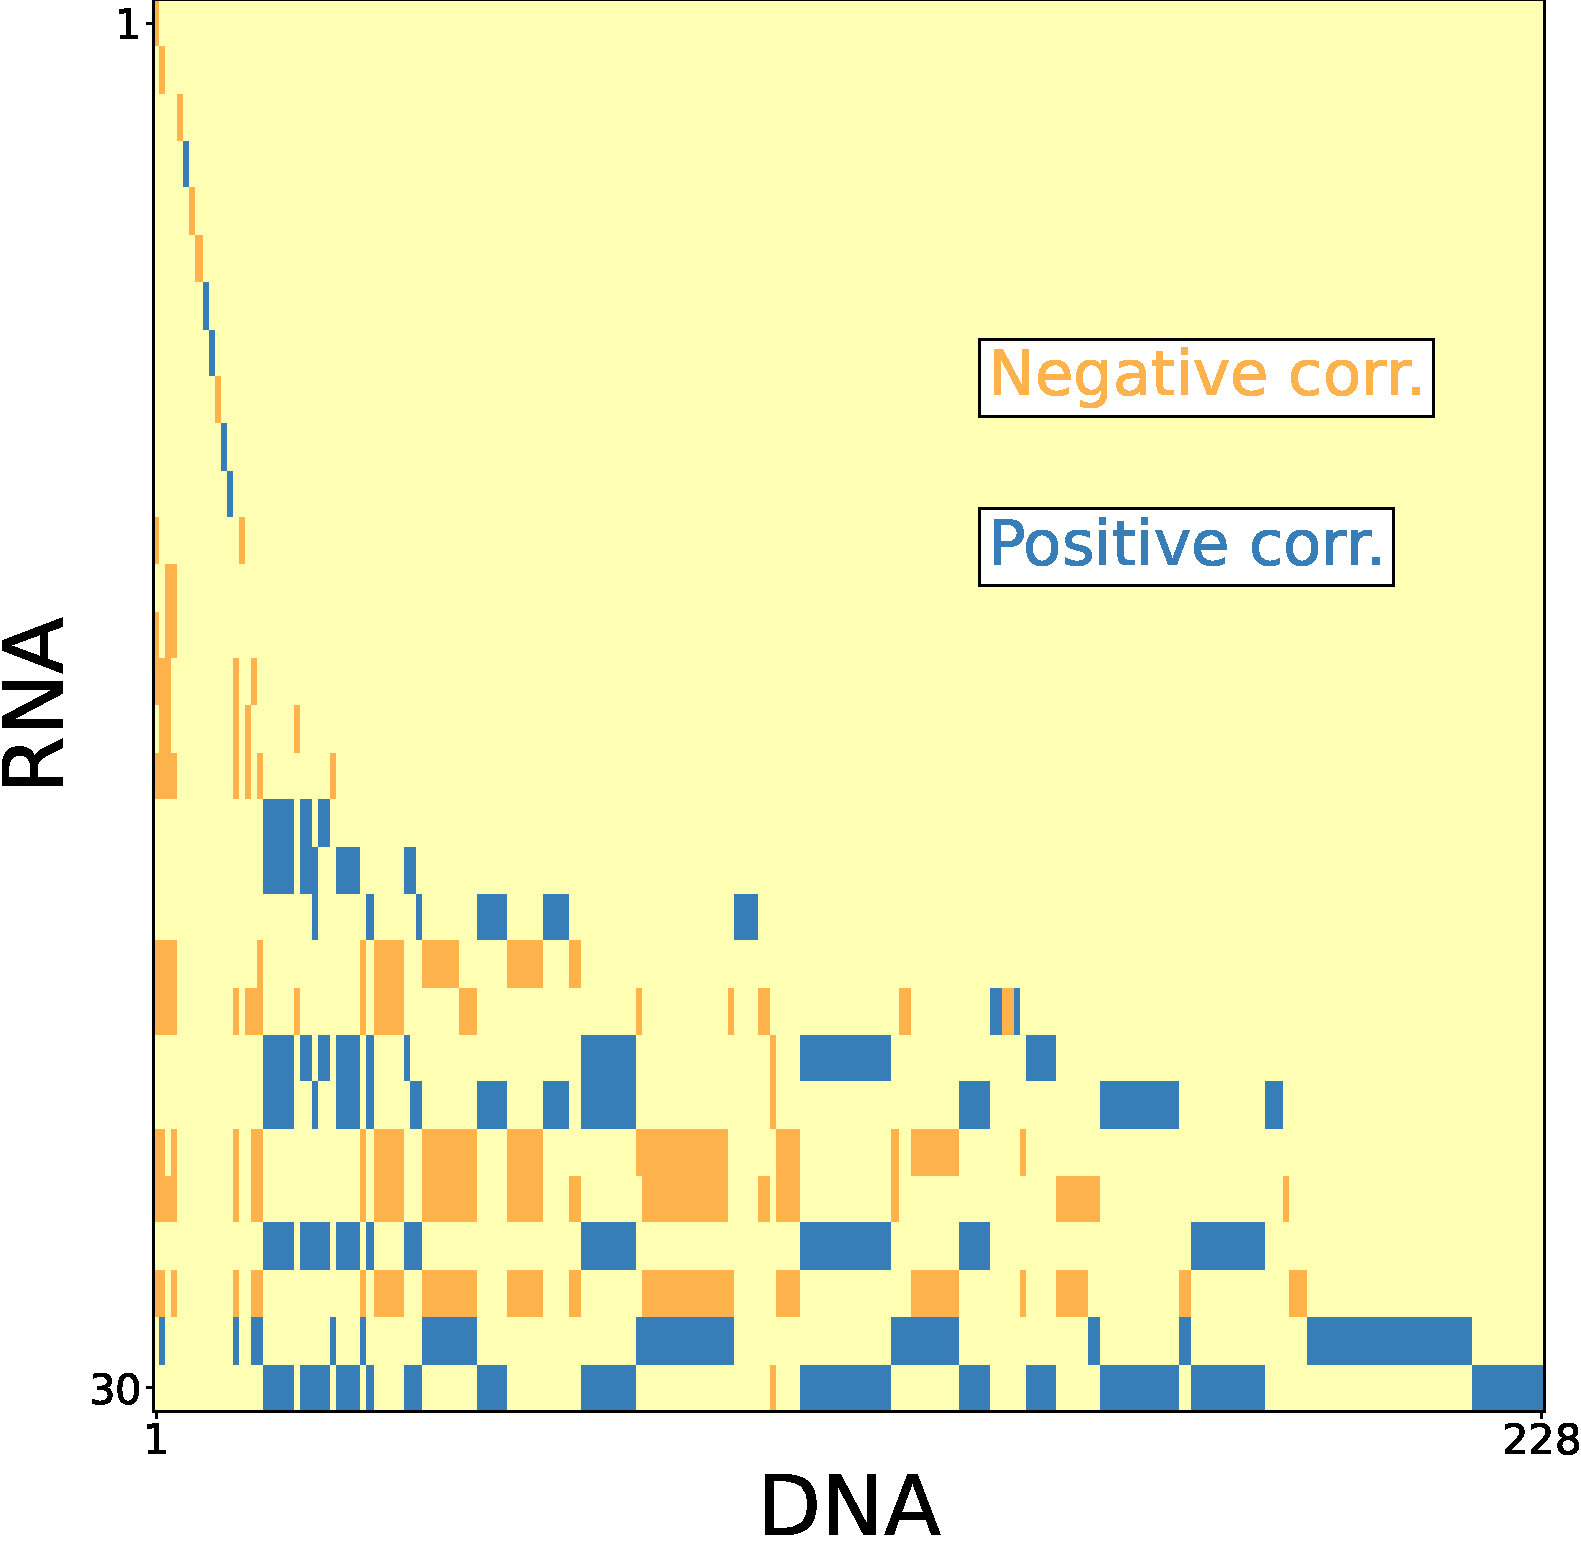
\includegraphics[width=0.5\columnwidth]{FIG/ADN_c-ARN_FQ-Matrix-sum-unit-0.7-PN.pdf}
}
\end{center}
\begin{center}
\resizebox{0.7\columnwidth}{!}{%
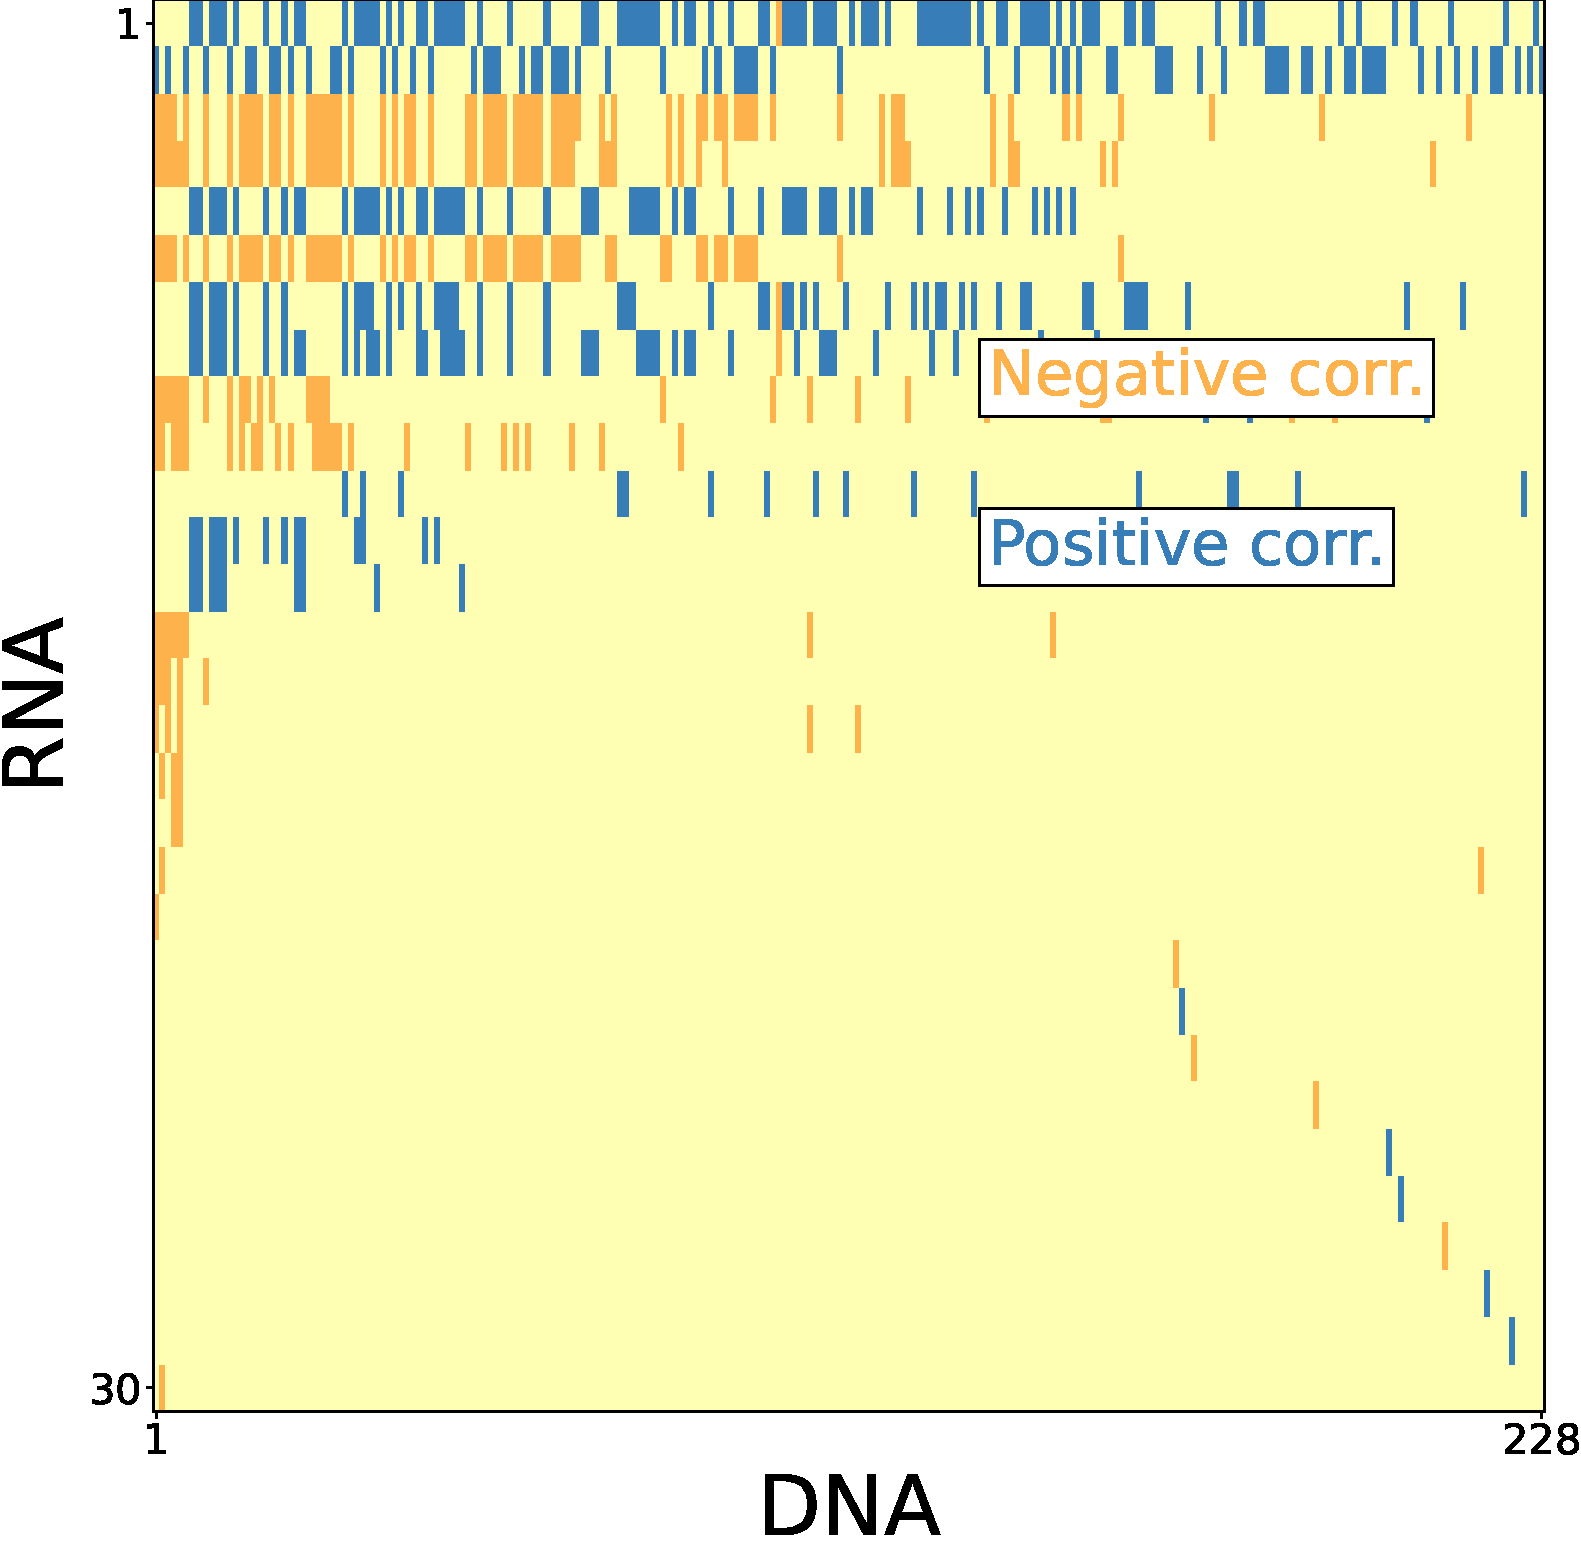
\includegraphics[width=0.5\columnwidth]{FIG/ADN_c-ARN_Degree-Matrix-unit-0.7-PN.pdf}
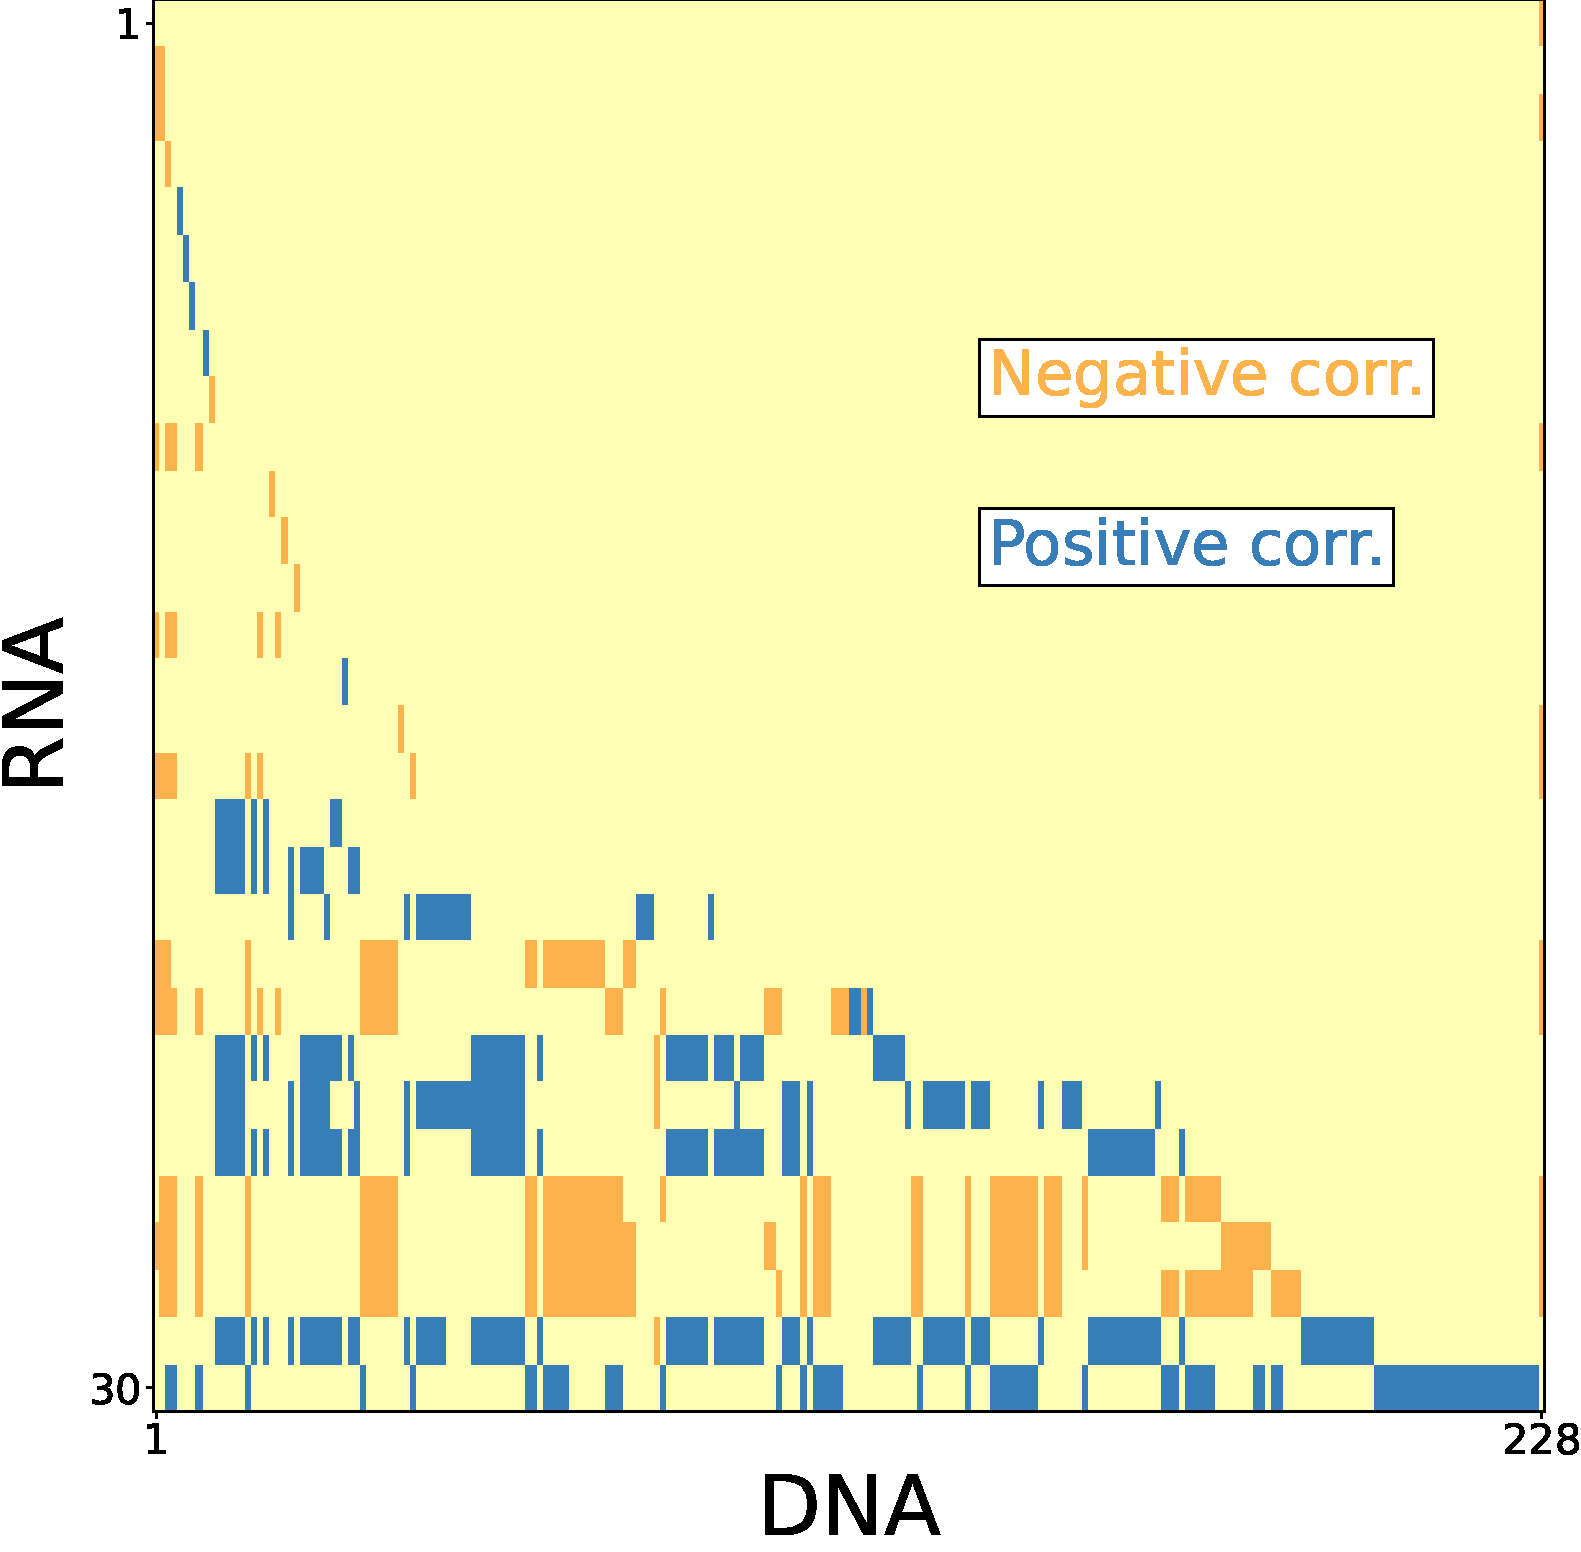
\includegraphics[width=0.5\columnwidth]{FIG/ADN_c-ARN_BINMATNEST-ESR1-Matrix-sum-unit-0.7-PN.pdf}
%\end{center}
}
\end{center}
\caption{\label{fig:fig1}Binary bi-adjacency matrix representing the interactions between Clustered DNAs and RNAs involved in ESR1 synthesis and regulation. Matrix entries related to positive correlations are in blue, and negative in orange, finally empty cells are in bright yellow. Raw matrix (top left), Fitness and Complexity based reorganized matrix (top right), Degree based reorganized matrix (bottom left) and matrix with cols and rows reorganized from BINMATNEST algorithm. Here we have considered all Pearson correlation such that $\rho_{c} = 0.7$.}
\end{figure}
 \begin{table}[h!]
\centering
\caption{\label{tab:tab1} Top 10 DNAs and RNAs in terms of fitness and complexity scores, 30 RNAs and 228 Clusters, with $\rho_{c} = 0.7$.}
\begin{tabular}{l|rr|rr|}
\cline{1-5}
RANK & CLUSTER ID & Fitness Score & RNA & Complexity Score\\
\cline{1-5}
1 & Cluster 91401 & 0.0779 & MYB & 0.0770\\
2 & Cluster 226 & 0.0556 & FSIP1 & 0.0755\\
3 & Cluster 62518 & 0.0501 & SRARP & 0.0739\\
4 & Cluster 20099 & 0.0373 & B3GALT1 & 0.07389\\
5 & Cluster 10765 & 0.0321 & PDZK1 & 0.07389\\
6 & Cluster 11329 & 0.0321 & SCNN1A & 0.0739\\
7 & Cluster 14885 & 0.0321 & ID4 & 0.0739\\
8 & Cluster 42066 & 0.0321 & SVEP1 & 0.0739\\
9 & Cluster 53084 & 0.0321 & CALML5 & 0.0739\\
10 & Cluster 55962 & 0.0321 & PTH1R & 0.0739\\
\cline{1-5}
\end{tabular}
\end{table}
 \begin{table}[h!]
\centering
\caption{\label{tab:tab2} Last 10 DNAs and RNAs in terms of fitness and complexity scores, 30 RNAs and 228 Clusters, with $\rho_{c} = 0.7$.}
\begin{tabular}{l|rr|rr|}
\cline{1-5}
RANK & CLUSTER ID & Fitness Score & RNA & Complexity Score\\
\cline{1-5}
1 & Cluster 83419 & 0.0004 & SIT1 & 0.0008\\
2 & Cluster 74585 & 0.0004 & MID1 & 0.0011\\
3 & Cluster 66780 & 0.0004 & FOXA1 & 0.0012\\
4 & Cluster 58323 & 0.0004 & CCR7 & 0.0013\\
5 & Cluster 55730 & 0.0004 & MLPH & 0.0013\\
6 & Cluster 49933 & 0.0004 & PRR15 & 0.0014\\
7 & Cluster 48271 & 0.0004 & IRF4 & 0.0015\\
8 & Cluster 24558 & 0.0004 & ICOS & 0.0017\\
9 & Cluster 24467 & 0.0004 & ESR1 & 0.0027\\
10 & Cluster 22095 & 0.0004 & TTC6 & 0.0031\\
\cline{1-5}
\end{tabular}
\end{table}
\begin{table}[h!]
\centering
\caption{\label{tab:tab3}Nestedness scores of the network obtained from $\rho_{c} = 0.7$. The NODF (BINMATNEST) score goes from $0$ (form $100$) for non nested network to $1$ ( to $0$) for highly nested network.}
\begin{tabular}{|r|r|}
\cline{1-2}
NODF & Temperature\\
\cline{1-2}
0.3 & 4.4\\
\cline{1-2}
\end{tabular}
\end{table}
\begin{figure}[h!]
%\begin{center}
\begin{center}
\resizebox{0.7\columnwidth}{!}{%
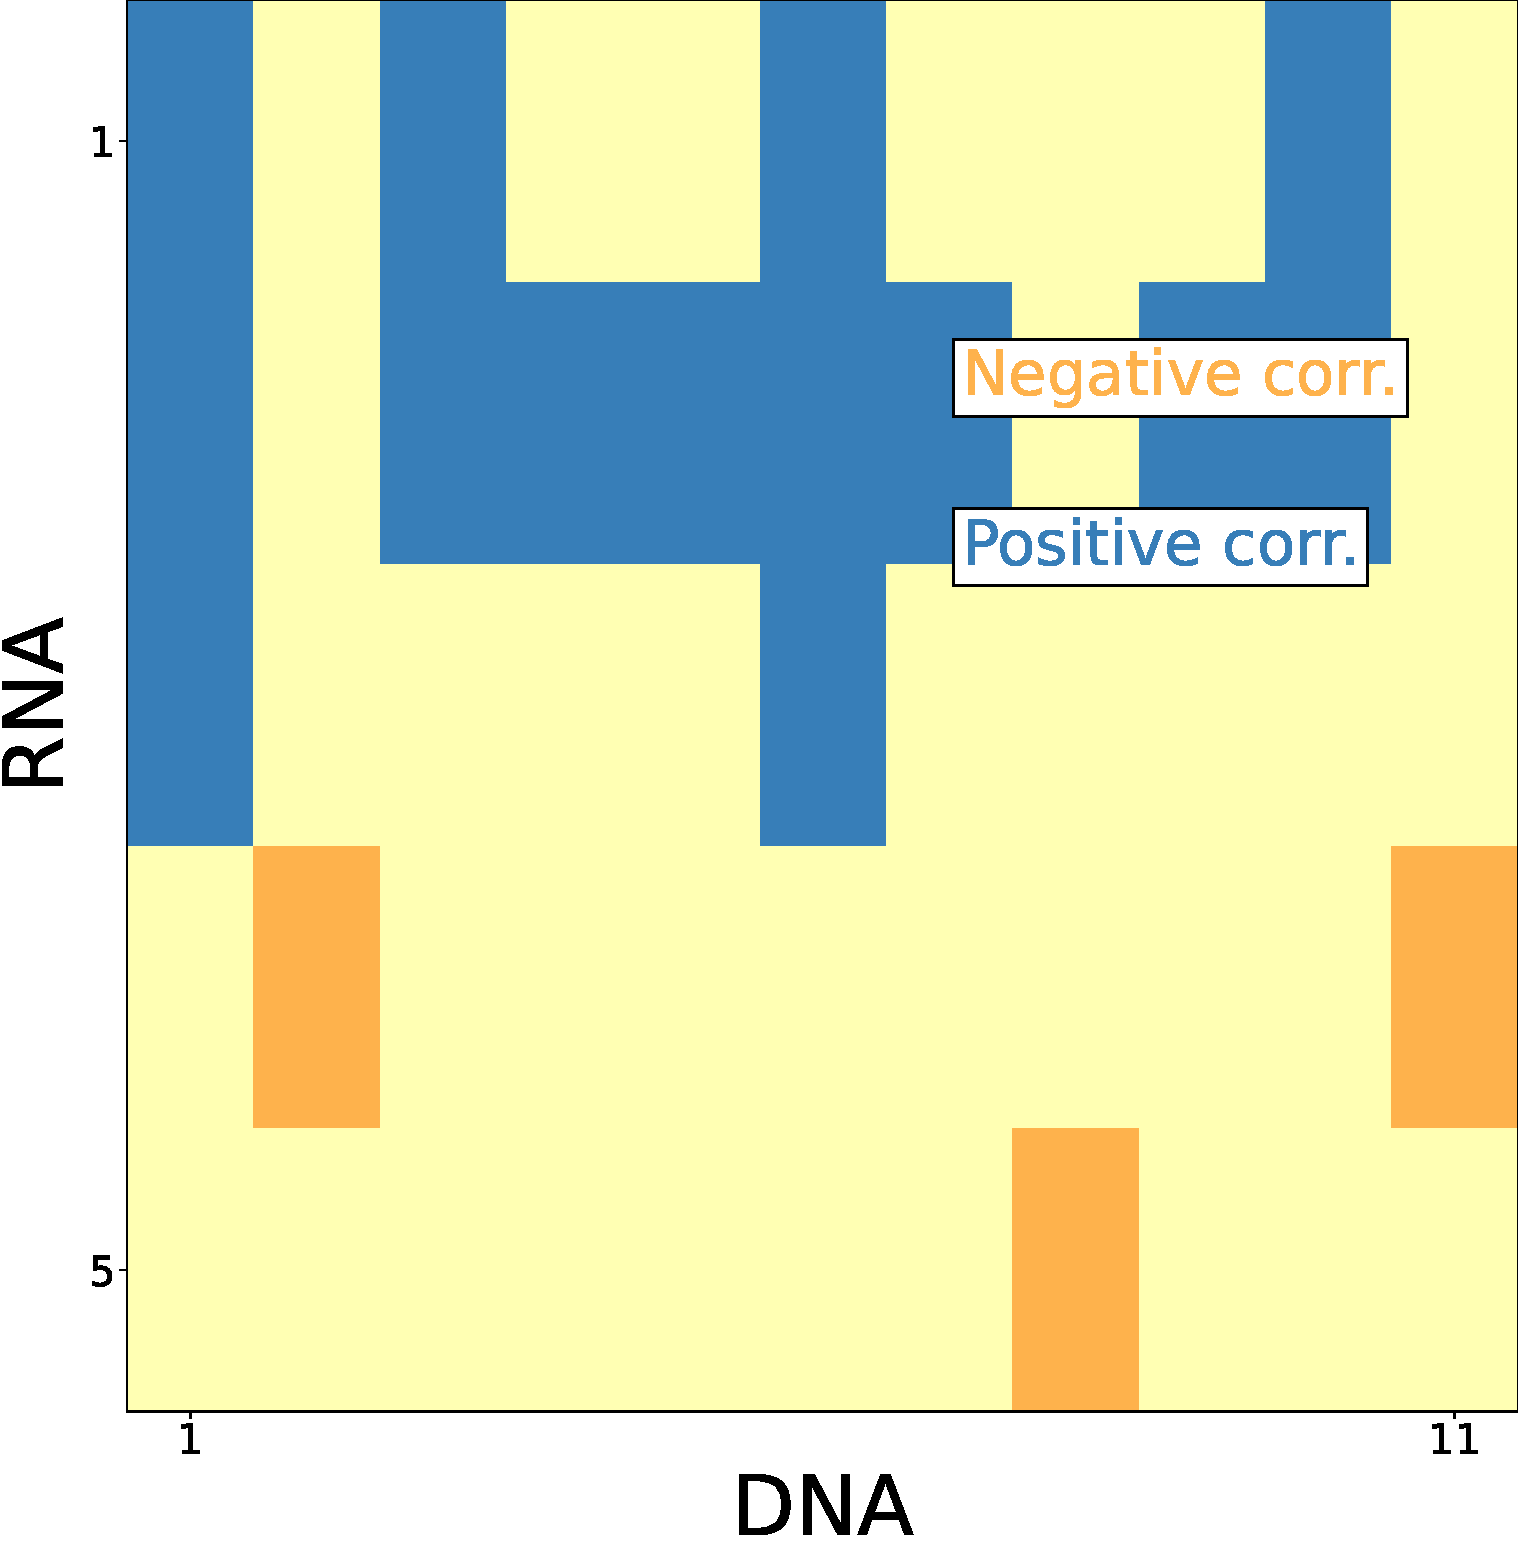
\includegraphics[width=0.5\columnwidth]{FIG/ADN_c-ARN_Matrix-unit-0.8-PN.pdf}
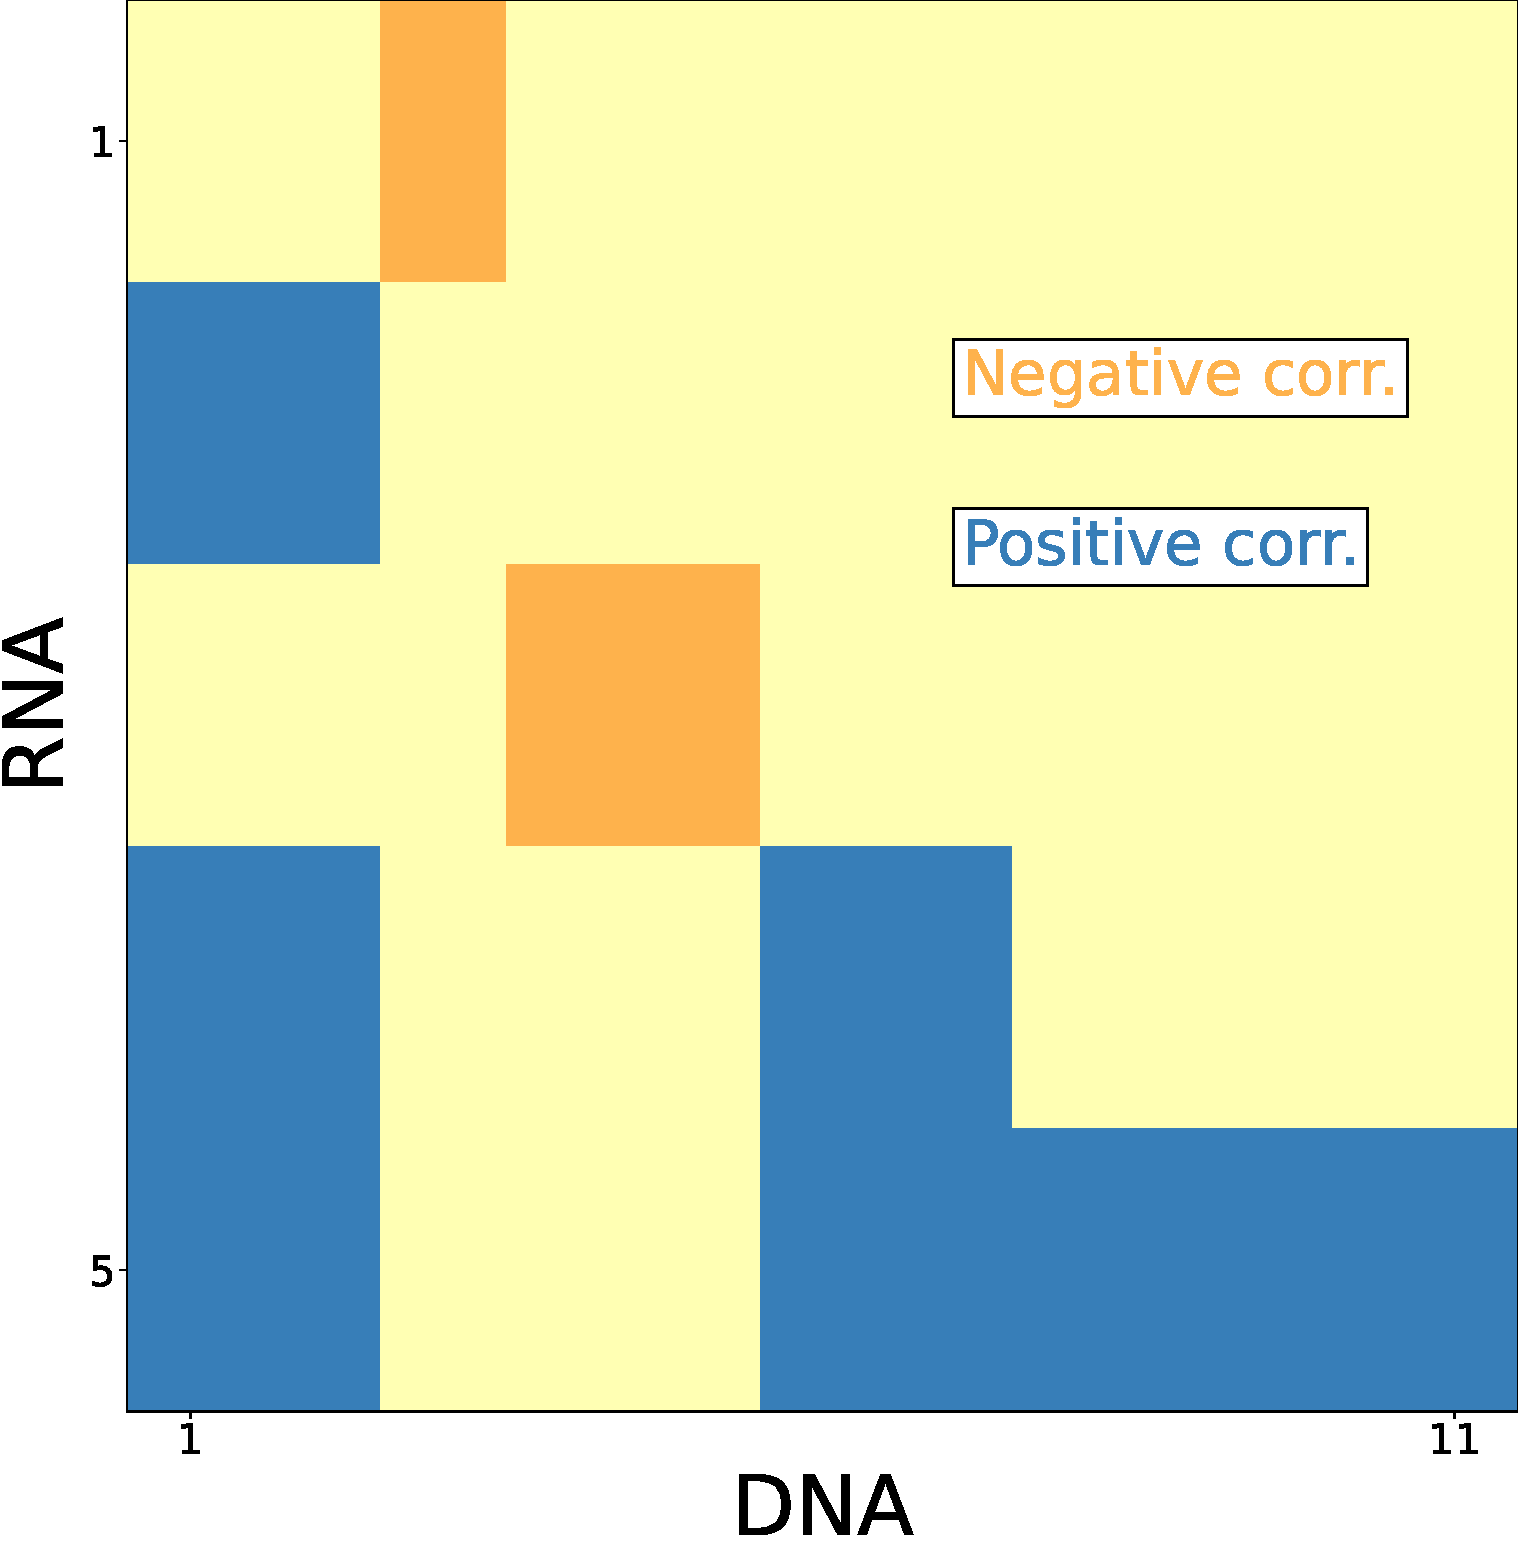
\includegraphics[width=0.5\columnwidth]{FIG/ADN_c-ARN_FQ-Matrix-sum-unit-0.8-PN.pdf}
}
\end{center}
\begin{center}
\resizebox{0.7\columnwidth}{!}{%
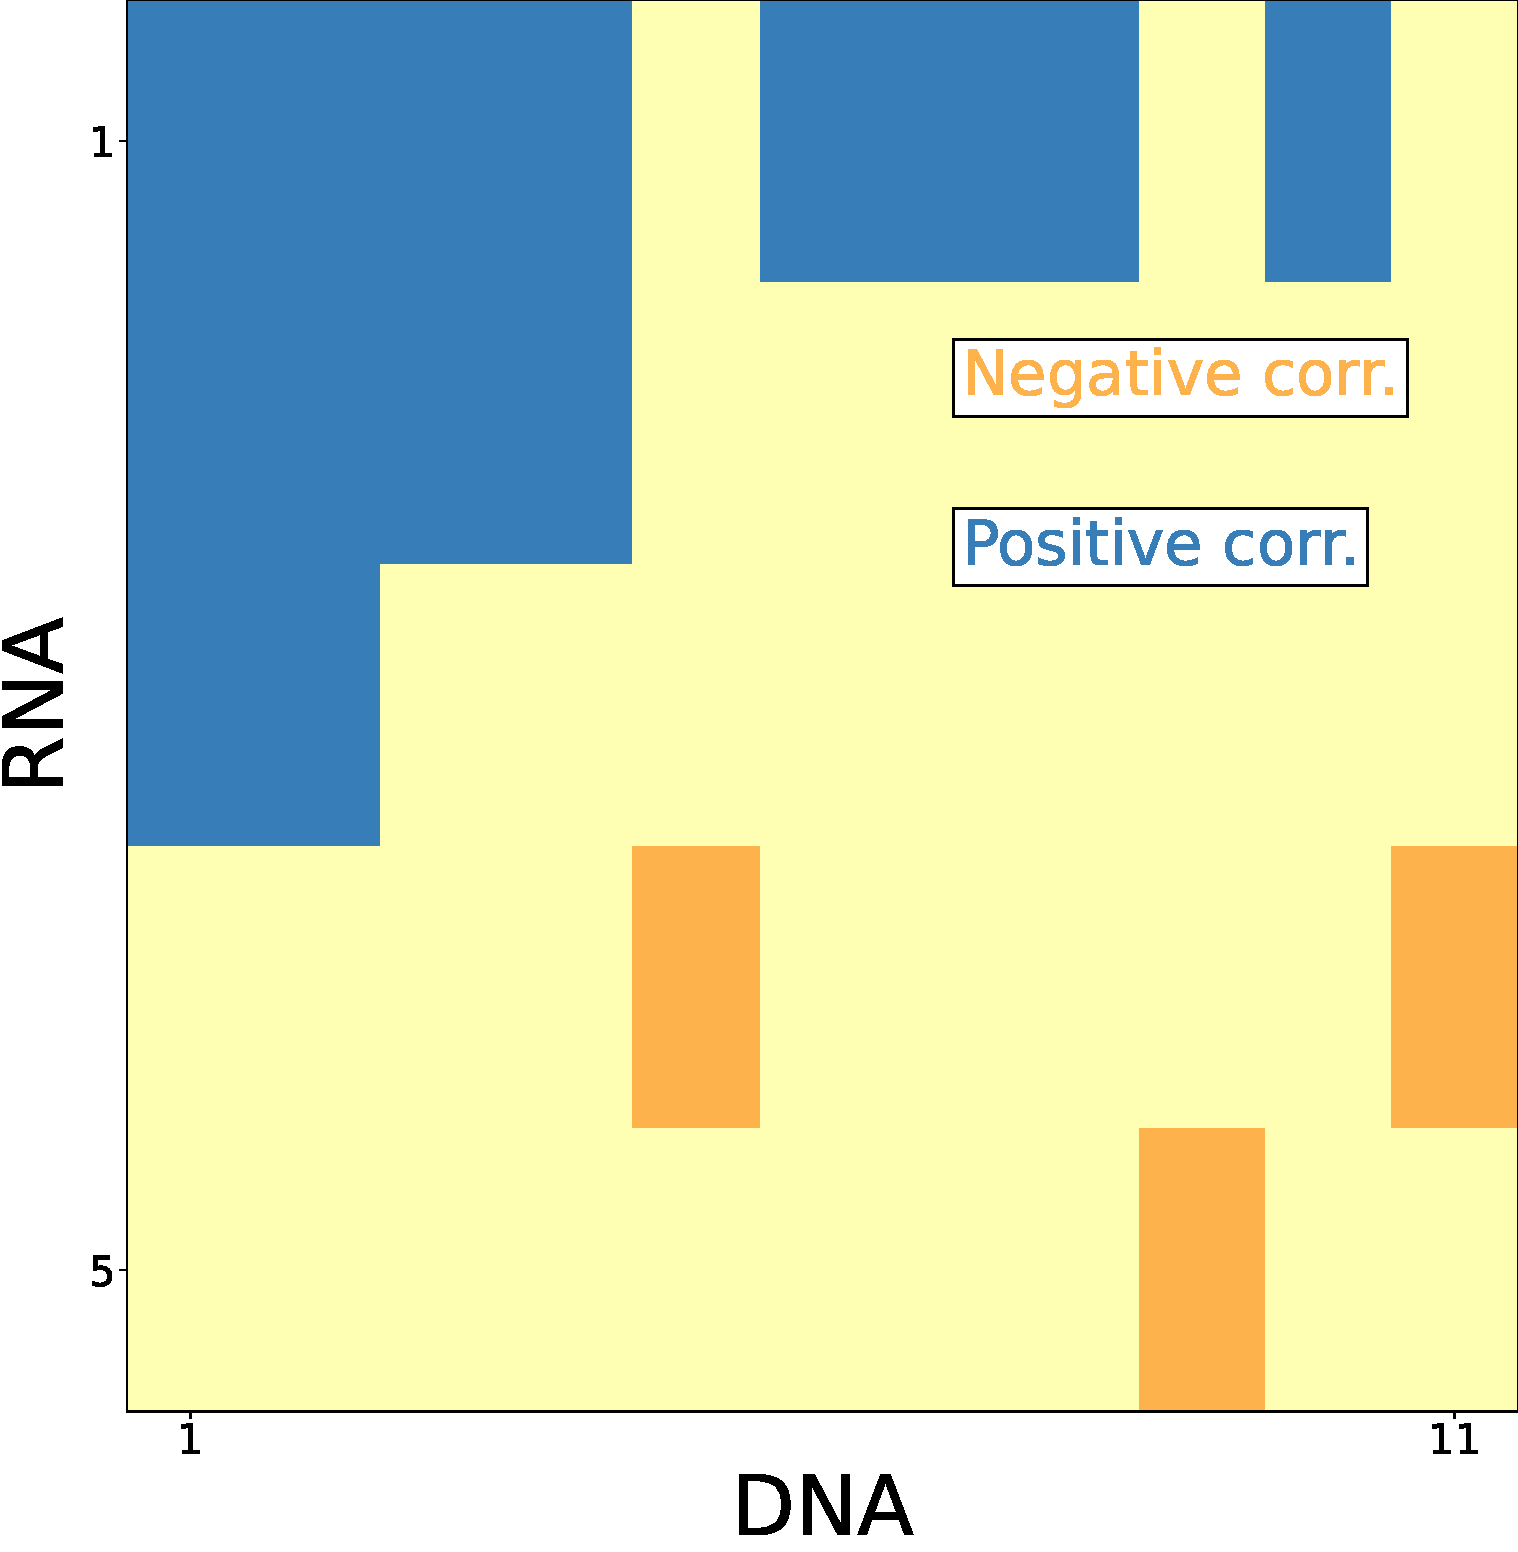
\includegraphics[width=0.5\columnwidth]{FIG/ADN_c-ARN_Degree-Matrix-unit-0.8-PN.pdf}
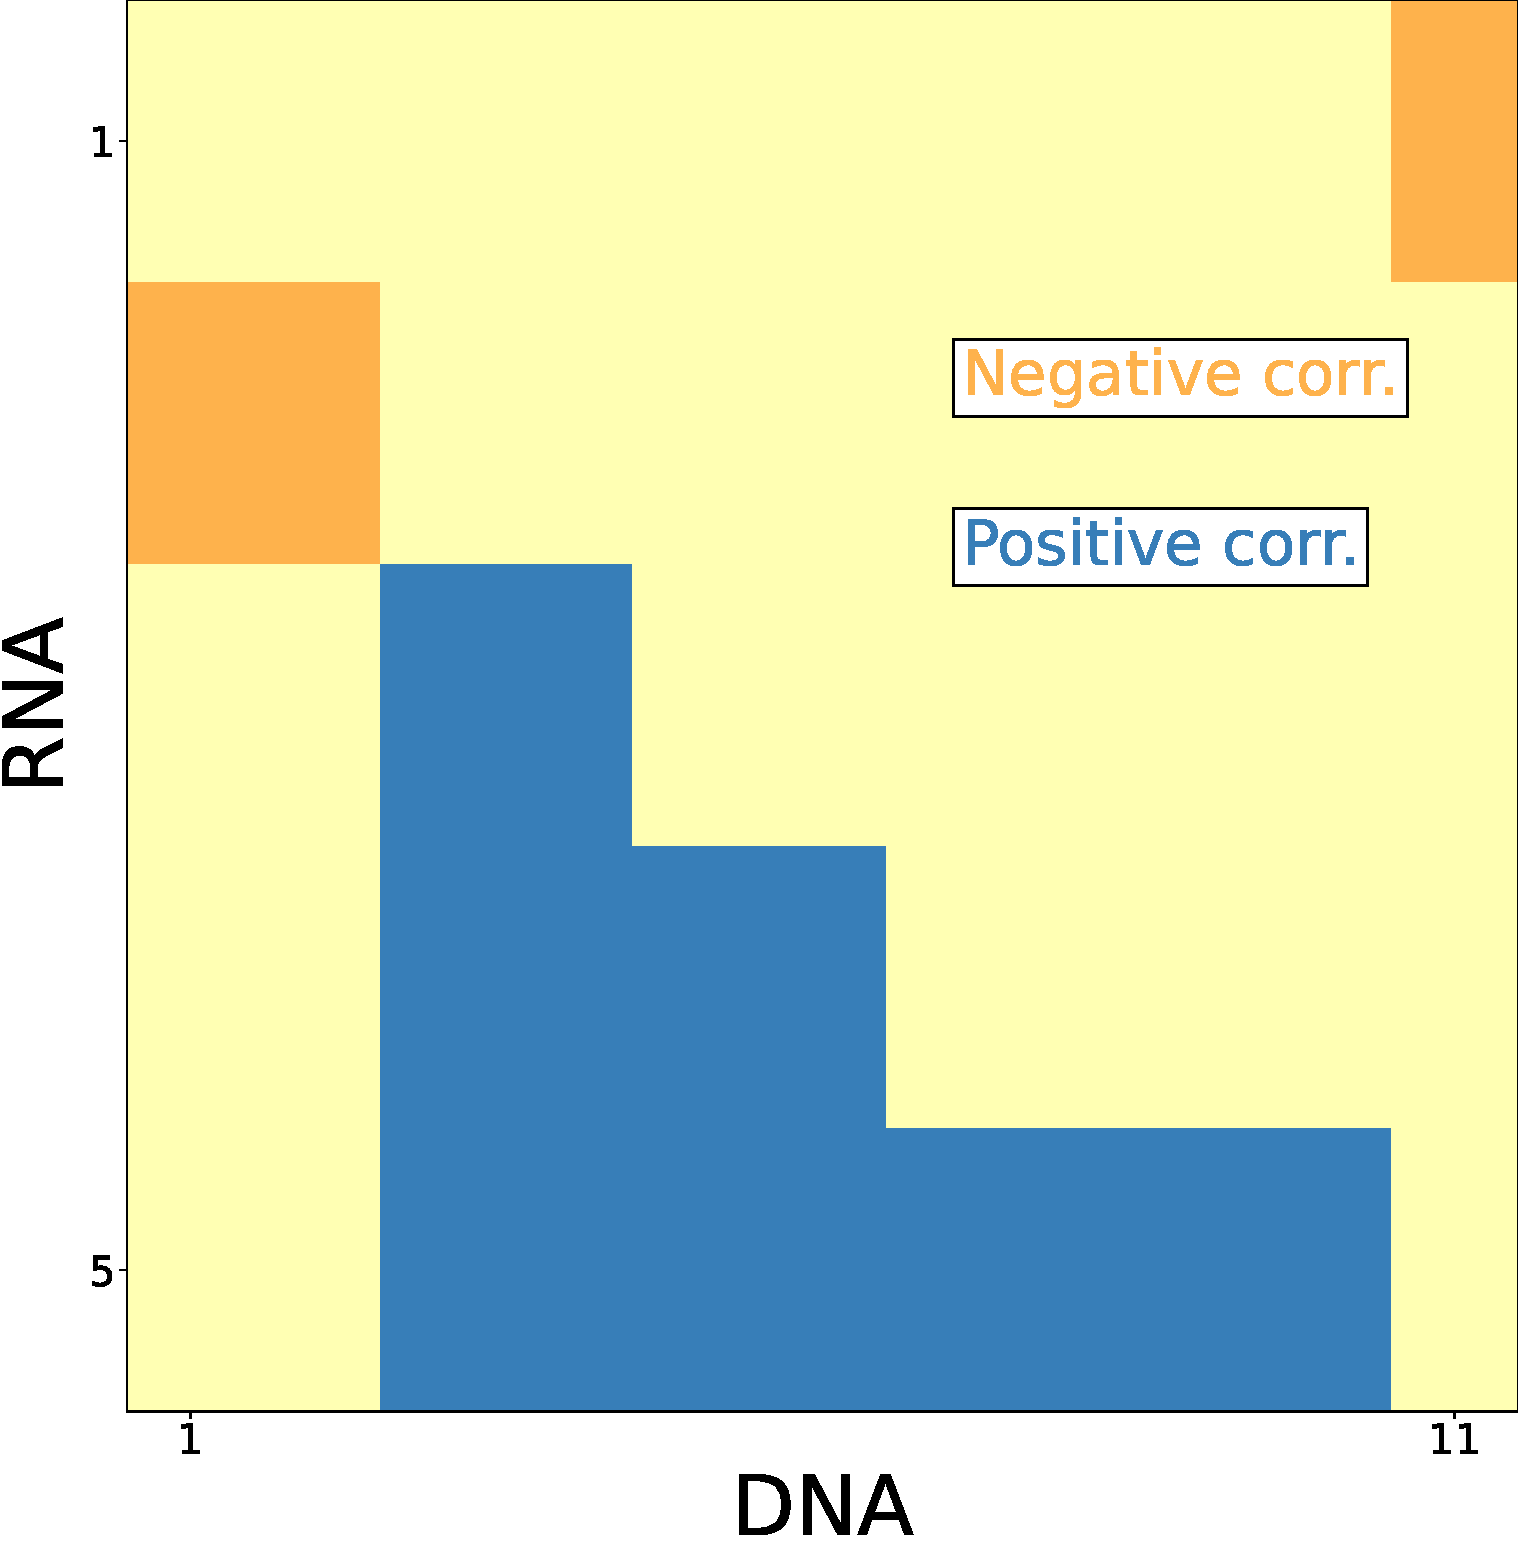
\includegraphics[width=0.5\columnwidth]{FIG/ADN_c-ARN_BINMATNEST-ESR1-Matrix-sum-unit-0.8-PN.pdf}
%\end{center}
}
\end{center}
\caption{\label{fig:fig2}Binary bi-adjacency matrix representing the interactions between Clustered DNAs and RNAs involved in ESR1 synthesis and regulation. Matrix entries related to positive correlations are in blue, and negative in orange, finally empty cells are in bright yellow. Raw matrix (top left), Fitness and Complexity based reorganized matrix (top right), Degree based reorganized matrix (bottom left) and matrix with cols and rows reorganized from BINMATNEST algorithm. Here we have considered all Pearson correlation such that $\rho_{c} = 0.8$.}
\end{figure}
 \begin{table}[h!]
\centering
\caption{\label{tab:tab4} All Clustered DNAs and RNAs in terms of fitness and complexity scores, 5 RNAs and 11 Clusters, with $\rho_{c} = 0.8$.}
\begin{tabular}{l|rr|rr|}
\cline{1-5}
RANK & CLUSTER ID & Fitness Score & RNA & Complexity Score\\
\cline{1-5}
1 & Cluster 11394 & 0.187 & ESR1 & 0.365\\
2 & Cluster 34909 & 0.187 & ICOS & 0.236\\
3 & Cluster 78422 & 0.163 & FOXA1 & 0.217\\
4 & Cluster 18269 & 0.097 & CCR7 & 0.122\\
5 & Cluster 91401 & 0.097 & SIT1 & 0.059\\
6 & Cluster 18410 & 0.081 & & \\
7 & Cluster 83354 & 0.081 & &\\
8 & Cluster 30403 & 0.026 & & \\
9 & Cluster 33345 & 0.026 & & \\
10 & Cluster 42067 & 0.026 & & \\
11 & Cluster 79424 & 0.026 & & \\
\cline{1-5}
\end{tabular}
\end{table}
\begin{table}[h!]
\centering
\caption{\label{tab:tab5}Nestedness scores of the network obtained from $\rho_{c} = 0.8$. The NODF (BINMATNEST) score goes from $0$ (form $100$) for non nested network to $1$ ( to $0$) for highly nested network.}
\begin{tabular}{|r|r|}
\cline{1-2}
NODF & Temperature\\
\cline{1-2}
0.3 & 16.3\\
\cline{1-2}
\end{tabular}
\end{table}
\clearpage
\printbibliography
\end{document}	